\documentclass[a4paper, 12pt]{article}

\usepackage{hyperref}
\usepackage[warn]{mathtext}
\usepackage[utf8]{inputenc}
\usepackage[T2A]{fontenc}
\usepackage[english,russian]{babel}
\usepackage{multirow}
\usepackage{amsmath,amsfonts,amssymb,amsthm,mathtools}
\usepackage{indentfirst}
\DeclareSymbolFont{T2Aletters}{T2A}{cmr}{m}{it}
\usepackage{ gensymb }
\mathtoolsset{showonlyrefs=true}
\usepackage{euscript}
\usepackage{mathrsfs}
\usepackage[left=2cm,right=2cm,top=2cm,bottom=2cm]{geometry}
\usepackage{graphicx}
\usepackage{wrapfig}
\usepackage[rgb]{xcolor}
\hypersetup{
colorlinks=true,
urlcolor=blue
}

\title{Лабораторная работа}
\author{Гисич Арсений Б03-102}
\date{2022}

\begin{document}

	\begin{center}
		{\large МОСКОВСКИЙ ФИЗИКО-ТЕХНИЧЕСКИЙ ИНСТИТУТ (НАЦИОНАЛЬНЫЙ ИССЛЕДОВАТЕЛЬСКИЙ УНИВЕРСИТЕТ)}
	\end{center}
	\vspace{5 cm}
	{\Large
		\begin{center}
			{\bf Лабораторная работа 3.2.3}\\[0.2 cm]
			Резонанс токов в параллельном контуре
		\end{center}
	}
	\vspace{4 cm}
	\begin{flushright}
		{\Large Выполнил: \\
			\vspace{0.2 cm}
			Гисич Арсений \\
			\vspace{0.2 cm}
			Б03-102 \\}
	\end{flushright}
	\vspace{9 cm}
	\begin{center}
		Долгопрудный\\[0.1 cm]
		2022
	\end{center}
\thispagestyle{empty}

\section{Аннотация}

В данной работе исследовался резонанс токов в параллельном колебательном контуре с изменяемой ёмкостью, были получены амплитудно-частотные и фазово-частотные характеристики, определены основные параметры контура.

\section{Теоретические сведения}

\begin{wrapfigure}{r}{0.3\textwidth}
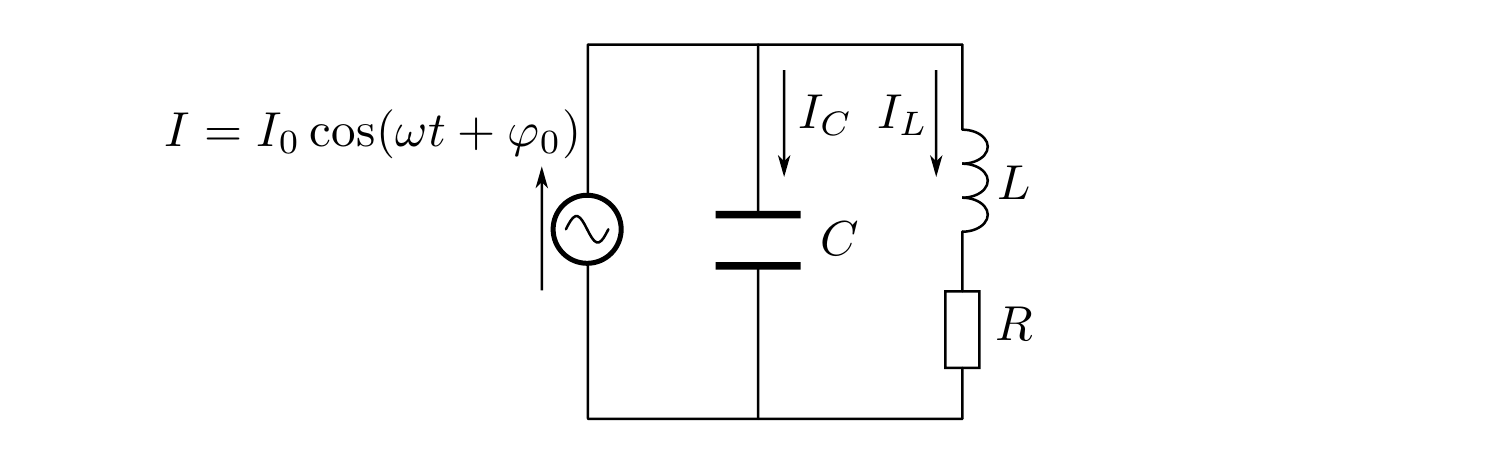
\includegraphics[width=0.3\textwidth]{1.png}
\caption{Последовательный контур с внешней ЭДС}
\label{r1}
\end{wrapfigure}

Рассмотрим процессы, протекающие в контуре, подключённом к источнику внешней ЭДС, изменяющейся по гармоническому закону $\varepsilon = \varepsilon_0 \cos{(\omega t + \varphi_0)}$. Для напряжения на конденсаторе $U_C(t)$ получим уравнение 
\begin{equation}\label{eq1}
\ddot{U}_C + 2\gamma \dot{U}_C + \omega_0^2U_С = \varepsilon_0\cos{(\omega t + \varphi_0)}.
\end{equation}

Перейдём к комплексному представлению колебаний. Запишем уравнение~\eqref{eq1} в комплексной форме, обозначая комплексные величины как <<векторы>>:
\begin{align}\label{eq2}
U_C & = \mathrm{Re}\,\mathbf{U_C}, & \mathbf{U_C} & = \mathrm{Re}\,\mathbf{U_C} + i\,\mathrm{Im}\,\mathbf{U_C}, \\
\varepsilon & = \mathrm{Re}\,\mathbf{\varepsilon}, & \mathbf{\varepsilon} & = \mathbf{\varepsilon_0}e^{i\omega t} = \varepsilon_0e^{i(\omega t + \varphi_0)},
\end{align}
\begin{equation}\label{eq3}
\mathbf{\ddot{U}_C} + 2\gamma \mathbf{\dot{U}_C} + \omega_0^2\mathbf{U_С} = \omega_0^2\mathbf{\varepsilon}.
\end{equation}

Комплексный множитель $\mathbf{\varepsilon_0} = \varepsilon_0e^{i\varphi_0}$, стоящий перед $e^{i\omega t}$, называется \textit{комплексной амплитудой}.

Решив уравнение~\eqref{eq3}, получим комплескное выражение для напряжения на конденсаторе $\mathbf{U_C}$. \textit{Вещественная часть} этого решения $\mathrm{Re}\,\mathbf{U_C}$ и является решением исходного уравнения~\eqref{eq1}. Будем искать решение уравнения~\eqref{eq3} в виде
\begin{equation}\label{eq4}
\mathbf{U_C}(t) = \mathbf{U_{C0}}e^{i\omega t},
\end{equation}
где $\mathbf{U_{C0}}$ --- комплексная амплитуда напряжения на конденсаторе, не зависящая от времени. Подставляя \eqref{eq4} в \eqref{eq3}, находим $\mathbf{U_{C0}}$ и далее, комплексные амплитуды тока в контуре и напряжений на сопротивлении и индуктивности:
\begin{equation}\label{eq5}
\mathbf{U_{C0}} = \frac{\mathbf{\varepsilon_0}}{i\omega CZ}, \quad Z = R + i\left(\omega L - \frac{1}{\omega C}\right),
\end{equation}
\begin{equation}\label{eq6}
\mathbf{I_0} = \frac{\mathbf{\varepsilon_0}}{Z}, \quad \mathbf{U_{R0}} = \frac{R\mathbf{\varepsilon_0}}{Z}, \quad \mathbf{U_{L0}} = i\omega L\frac{\mathbf{\varepsilon_0}}{Z}.
\end{equation}

Комплексная величина $Z$ называется \textit{комплексным сопротивлением}, или \textit{импедансом}, последовательного контура. Можно определить импеданс каждого отдельного элемента контура:
\begin{equation}\label{eq7}
Z_R = R, \quad Z_L = i\omega L, \quad Z_C = \frac{1}{i\omega C}.
\end{equation}

В новых обозначениях уравнения \eqref{eq5}--\eqref{eq6} принимают вид
\begin{equation}\label{eq8}
\mathbf{I} = \frac{\mathbf{\varepsilon_0}}{Z}, \quad \mathbf{U_{R0}} = Z_R\mathbf{I_0}, \quad \mathbf{U_{C0}} = Z_C\mathbf{I_0}, \quad \mathbf{U_{L0}} = Z_L\mathbf{I_0}.
\end{equation}

Импеданс контура $Z$ не зависит от начальных условий, не содержит величин ни токов, ни напряжений, а определяется свойствами всех элементов, соединённых в контур, и частотой синусоидальной ЭДС, к которой он подключён. Таким образом, \textit{импеданс $Z$ является характеристикой колебательного контура на заданной частоте}.

Выражение \eqref{eq5} для импеданса контура $Z$ содержит действительную часть $$\mathrm{Re}\,Z = R,$$ называемую \textit{активным} сопротивлением контура, и мнимую часть $$\mathrm{Im}\,Z = \omega L - \frac{1}{\omega C},$$ носящую название \textit{реактивного} сопротивления.

Импедансы контура и его отдельных элементов --- комплексные числа --- могут быть представленны в показательной форме:
\begin{equation}\label{eq9}
Z = Z_0e^{i\psi},
\end{equation}
где $Z_0 = |Z|$ --- модуль комплексного числа, $\psi = \arg{Z}$ --- его аргумент (фаза). Для импеданса рассматриваемого последовательного контура при этом находим
\begin{equation}\label{eq10}
Z_0 = \sqrt{(\mathrm{Re}\,Z)^2 + (\mathrm{Im}\,Z)^2} = \sqrt{R^2 + \left(\omega L - \frac{1}{\omega C}\right)^2} = \frac{R}{\cos{\psi_I}},
\end{equation}
\begin{equation}\label{eq11}
\tan{\psi_I} = \frac{\mathrm{Im}\,Z}{\mathrm{Re}\,Z} = \frac{\omega L - \frac{1}{\omega C}}{R}.
\end{equation}
Ток в контуре и напряжения на отдельных его элементах теперь могут быть получены по формулам~\eqref{eq5}--\eqref{eq8}. Например, действительная часть тока в контуре
\begin{equation}\label{eq12}
I(t) = \frac{\varepsilon_0}{R}\cos{\psi_I}\cos({\omega t + \varphi_0 - \psi_I)}.
\end{equation}
Как видно из~\eqref{eq11}~и~\eqref{eq12}, угол~$\psi_I$, определяемый отношением мнимой и действительной частей импеданса, представляют собой сдвиг фаз между напряжением на последовательном контуре и током в нём, причём \textit{положительные значения угла~$\psi_I$ соответствуют отставанию фазы тока, а отрицательные --- опережению}. В общем случае, когда к источнику последовательно подключены резистор, конденсатор и катушка самоиндукции, сдвиг фазы $\psi_I$ лежит в пределах $-\pi/2 < \psi_I < \pi/2$.

\section{Методика измерений}

\textbf{\begin{figure}[h!]
\begin{center}
    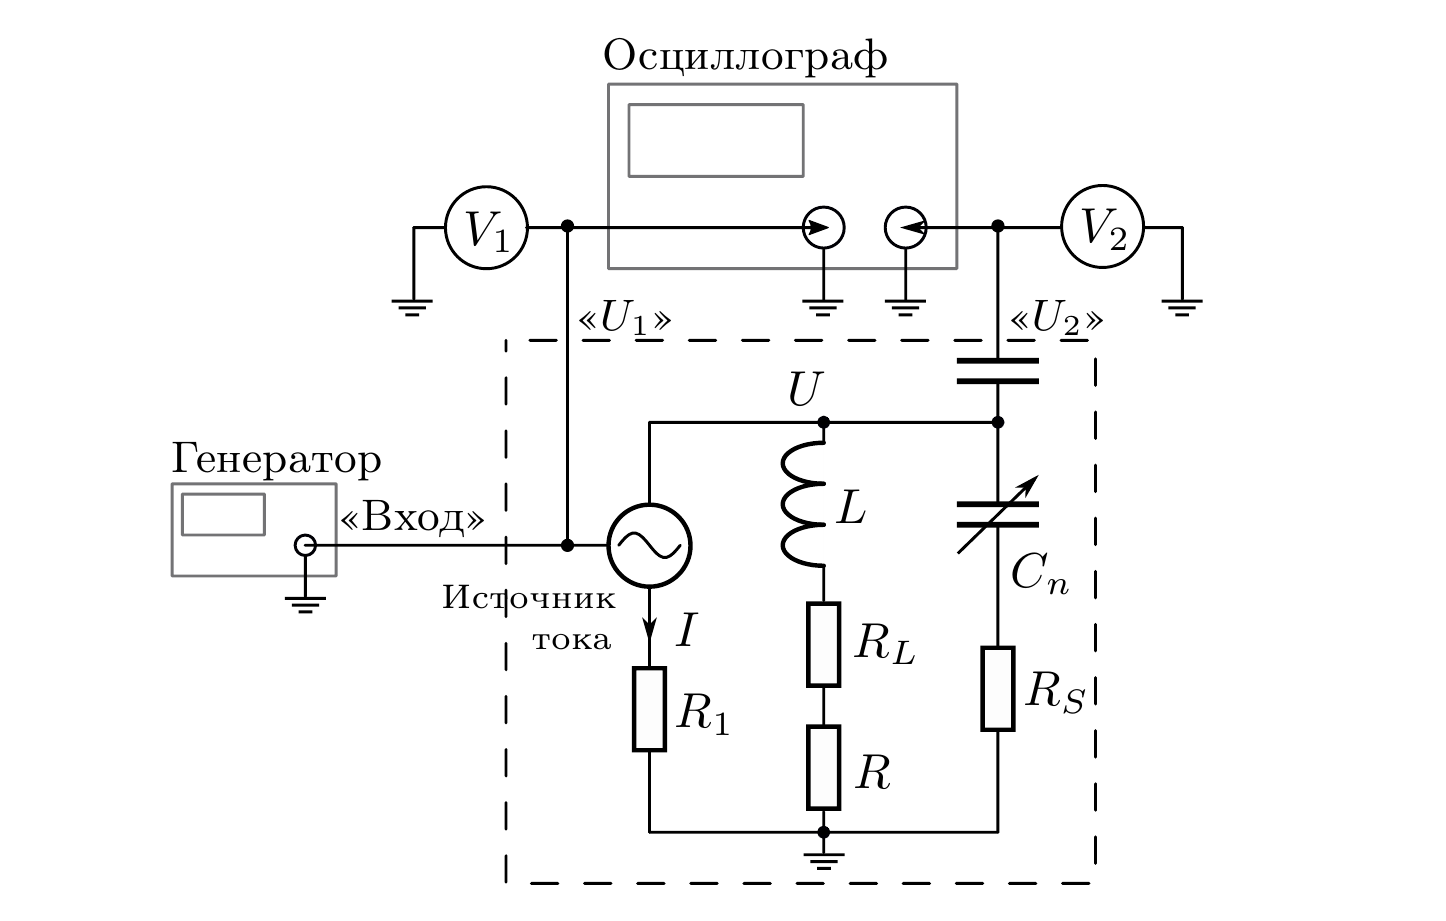
\includegraphics[scale=2.5]{ust.png}
\end{center}
\caption{Блок-схема экспериментального стенда}
\label{ust}
\end{figure}}

$I=\dfrac{E}{R_I}=\dfrac{E_0cos(\omega t+\varphi_0)}{R_I}=I_0cos(\omega t+\varphi_0)$ --- ток на генераторе\newline
$$R_S=\dfrac{U_{RS}}{I}=\frac{U_{RS}}{\omega CU_{CS}}=\dfrac{1}{\omega C}tg\delta$$
где $R_S$ --- эквивалентное последовательное сопротивление (ЭПС)\newline
Для используемых емкостей $C_n$ выполнено $tg\delta<10^{-3}$\newline
$$R_{\sum}=R+R_L+R_S$$
где $R_{\sum}$ --- суммарное активное сопротивление контура.\newline
Воспользуемся методом комплексных амплитуд:\newline
$Z_L=R_L+i\omega L$, $Z_C=R_S-i\frac{1}{\omega C}$, $Z=R_{\sum}+i(\omega L-d\dfrac{1}{\omega C})$\newline
Тогда напряжение на контуре и токи на индуктивной и емкостной частях контура при нулевой начальной фазе можно представить в виде:\newline
$$I_c=I\dfrac{Z_L}{Z_C+Z_L}=iQI_0\dfrac{\omega}{\omega_0}\dfrac{1-i\dfrac{R+R_L}{\rho}\dfrac{\omega_0}{\omega}}{1+iQ(\dfrac{\omega}{\omega_0}-\dfrac{\omega_0}{\omega})}$$
$$I_L=I\dfrac{Z_c}{Z_C+Z_L}=iQI_0\frac{\omega_0}{\omega}\frac{1+itg\delta}{1+iQ(\frac{\omega}{\omega_0}-\frac{\omega_0}{\omega})}$$
$$U=I\frac{Z_LZ_c}{Z_C+Z_L}=Q\rho I_0\frac{(1-i\frac{R+R_L}{\rho}\frac{\omega_0}{\omega})(1+itg\delta)}{1+iQ(\frac{\omega}{\omega_0}-\frac{\omega_0}{\omega})}$$
где $\omega_0=\frac{1}{\sqrt{LC}}$ --- собственная частота, $\rho=\sqrt{\frac{L}{C}}$ --- реактивное сопротивление контура, $Q=\frac{\rho}{R_{\sum}}$ --- добротность контура\newline
Рассмотрим случай, когда $|\Delta\omega|=|\omega-\omega_0|\ll\omega_0$. Тогда
$$\frac{\omega}{\omega_0}-\frac{\omega_0}{\omega}=\frac{2\Delta\omega}{\omega_0}$$
Пренебрегая поправками порядка $Q^{-2}$, получим:
$$I_c=QI_0\frac{\omega}{\omega_0}\frac{e^{i\phi_c}}{\sqrt{1+(\tau\Delta\omega)^2}},    \phi_c=\frac{\pi}{2}-\frac{R+R_L}{\rho}-arctg(\tau\Delta\omega)$$
$$I_L=QI_0\frac{\omega_0}{\omega}\frac{e^{i\phi_L}}{\sqrt{1+(\tau\Delta\omega)^2}}, \phi_L=-\frac{\pi}{2}+\delta\arctg(\tau\Delta\omega)$$
$$U=Q\rho I_0\frac{\omega}{\omega_0}\frac{e^{i\phi_U}}{\sqrt{1+(\tau\Delta\omega)^2}}, \phi_U=-\frac{\omega}{\omega_0}\frac{R+R_L}{\rho}+\delta-arctg(\tau\Delta\omega)$$
где $\tau=\frac{2L}{R_{\sum}}=\frac{2Q}{\omega_0}$ --- время затухания.\newline
При резонансе, т.е. когда $\Delta\omega=0$:
$$I_c(\omega_0)=QI_0, \phi_c(\omega_0)=\frac{\pi}{2}-\frac{R+R_L}{\rho}$$
$$I_L(\omega_0)=QI_0, \phi_L(\omega_0)=-\frac{\pi}{2}+\delta$$
$$U(\omega_0)=Q\rho I_0=Q^2R_{\sum}I_0, \phi_U{\omega_0}=-\frac{R+R_L}{\rho}+\delta$$
$$\phi'_c(\omega_0)=\phi'_L(\omega_0)=\phi'_U(\omega_0)=-\tau$$
  	
\section{Используемое оборудование}

\begin{enumerate}
    \item генератор сигналов;
    \item источник напряжения;
    \item двухканальный осциллограф;
    \item цифровые вольтметры;
\end{enumerate}

\section{Результаты измерений и обработка данных}

Параметры образца:
\begin{description}
\item{} $a = 2,2~мм$
\item{} $L = 6,0~мм$
\item{} $l = 7~мм$
\end{description}

Результаты измерения калибровочной зависимости поля $B$ от тока в электромагните $I_М$ представлены в таб.~\ref{tab1}. Калибровочный график зависимости представлен на рис.~\ref{plot1}.

\begin{table}[h!]
\begin{center}
\begin{tabular}{|c|c|c|c|}
\hline
$I_М, А$ & $\delta_{I_М}, А$ & $B, мТл$ & $\delta_B, мТл$ \\ \hline
0,000 & 0,020  & 17,7   & 1,9     \\ \hline
0,210 & 0,021  & 224,8  & 12,2    \\ \hline
0,500 & 0,023  & 521,8  & 27,1    \\ \hline
0,810 & 0,024  & 802,7  & 41,1    \\ \hline
1,020 & 0,025  & 929,4  & 47,5    \\ \hline
1,220 & 0,026  & 1016,2 & 51,8    \\ \hline
1,420 & 0,027  & 1072,1 & 54,6    \\ \hline
\end{tabular}
\end{center}
\caption{Калибровочная зависимость $B(I_М)$}
\label{tab1}
\end{table}

\section{Обсуждение результатов и выводы}

В данной работе была исследована зависимость ЭДС Холла от величины магнитного поля при различных значениях тока через образец. Были определены постоянная Холла, подвижность и концентрация носителей заряда в образце легированного германия. Полученные значения:
$$\boxed{R_H = (739\pm35) \cdot 10^{-6}~\frac{м^3}{Кл}, \quad n = (8,5\pm0,2) \cdot 10^{21}~\frac{1}{м^3}, \quad \mu = 1446\pm123~\frac{см^2}{В \cdot с}}$$

Табличное значение собственной концентрации носителей зарядов для германия $n_0 = 2,4 \cdot 10^{13}~\frac{1}{м^3}$. Это меньше полученного значения, что говорит о том, что данный образец германия содержит примеси. Основной вклад в погрешность вносит погрешность определения коэффициентов зависимости. Также на ошибку измерений может влиять зависимость концентрации основных носителей заряда от температуры, ярко выраженная в полупроводниках.

\end{document}
